\documentclass[12pt,a4paper,twoside,openright,titlepage,final]{article}
\usepackage{fontspec}
\usepackage{amsmath}
\usepackage{amsfonts}
\usepackage{amssymb}
\usepackage{makeidx}
\usepackage{graphicx}
\usepackage[hidelinks,unicode=true]{hyperref}
\usepackage[spanish,es-nodecimaldot,es-lcroman,es-tabla,es-noshorthands]{babel}
\usepackage[left=3cm,right=2cm, bottom=4cm]{geometry}
\usepackage{natbib}
\usepackage{microtype}
\usepackage{ifdraft}
\usepackage{verbatim}
\usepackage[obeyDraft]{todonotes}
\ifdraft{
	\usepackage{draftwatermark}
	\SetWatermarkText{BORRADOR}
	\SetWatermarkScale{0.7}
	\SetWatermarkColor{red}
}{}
\usepackage{booktabs}
\usepackage{longtable}
\usepackage{calc}
\usepackage{array}
\usepackage{caption}
\usepackage{subfigure}
\usepackage{footnote}
\usepackage{url}
\usepackage{tikz}
\usepackage{pdflscape}
\usepackage{minted}

\setsansfont[Ligatures=TeX]{texgyreadventor}
\setmainfont[Ligatures=TeX]{texgyrepagella}

%*******************************************************
%                 NO MODIFICAR
\newcommand*{\FSfont}[1]{%
  \fontencoding{T1}\fontfamily{#1}\selectfont}

\newlength{\tpheight}\setlength{\tpheight}{0.9\textheight}
\newlength{\txtheight}\setlength{\txtheight}{0.9\tpheight}
\newlength{\tpwidth}\setlength{\tpwidth}{0.9\textwidth}
\newlength{\txtwidth}\setlength{\txtwidth}{0.9\tpwidth}
\newlength{\drop}
%*******************************************************

% Crea una portada con los siguientes parámetros
%
% #1 : Título 
% #2 : Subtítulo
% #3 : Subsubtítulo
% #4 : Autor(es)
% #5 : Lugar
%

\newcommand*{\portada}[5]{
\begin{titlepage}
\begingroup
\vspace*{1cm}
\drop = 0.2\txtheight
\centering
\vfill
{\Huge \scshape #1}\\[\baselineskip]
{\Large \textbf{#2}}\\[\baselineskip]
{\Large \scshape #3}\\[\baselineskip]
\vspace*{0.3cm}
{\large \textit{#4}}\\[0.5\drop]

\includegraphics[scale=0.35]{./imagenes/logoURJC.jpg}
\vspace*{1.5cm}

{\large \scshape #5, \today} \par
\begin{center}
\end{center}
\vfill\null
\endgroup
\end{titlepage}
}
 %*****************************************************
 


\author{José Ignacio Escribano}

\title{Caso práctico II: Generación de variables aleatorias}

\setlength{\parindent}{0pt}

\begin{document}

\pagenumbering{alph}
\setcounter{page}{1}

\portada{Caso práctico II}{Simulación y Metaheurísticas}{Generación de variables aleatorias}{José Ignacio Escribano}{Móstoles}

\listoftables
\thispagestyle{empty}
\newpage

\listoffigures
\thispagestyle{empty}
\newpage

\tableofcontents
\thispagestyle{empty}
\newpage


\pagenumbering{arabic}
\setcounter{page}{1}

\section{Introducción}

En este caso práctico utilizaremos distintos métodos para generar variables aleatorias; tanto unidimensionales como multidimensionales. En el primer caso generaremos la distribución exponencial y la normal. En el caso multidimensional, generaremos la distribución normal bivariante.

\section{Resolución del caso práctico}

A continuación resolveremos cada una de las cuestiones planteadas.

\subsection{Cuestión 1}\label{cuestion:1}

Usando el comando \texttt{rnorm} generaremos 10, 100 y 10000 observaciones de una distribución normal de parámetros ($\mu = 3, \sigma^2 = 6^2$).\\

La Figura~\ref{fig:Rplot} muestra los histogramas con cada número de muestras.\\

\begin{figure}[htbp!]
\centering
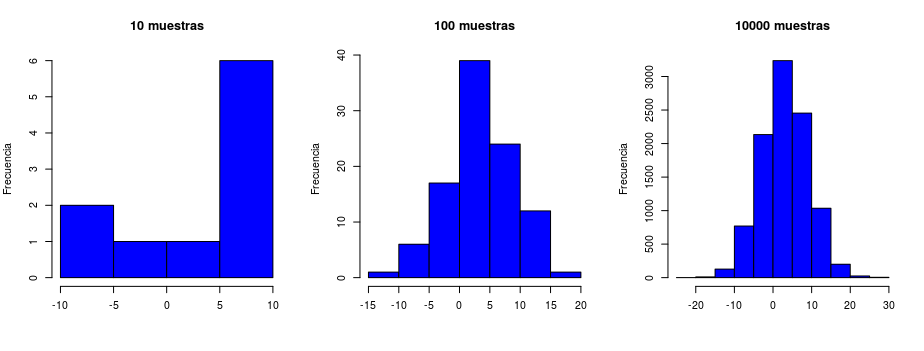
\includegraphics[width=0.8\linewidth]{imagenes/Rplot}
\caption{Histograma de una distribución normal con 10, 100 y 10000 muestras}
\label{fig:Rplot}
\end{figure}

Se puede observar como, a medida que se aumenta el número de muestras de la distribución, el histograma toma la forma característica de una distribución normal: simétrica y con forma de campana.\\

Usaremos distintos estadísticos muestrales para comprobar el hecho anterior. Estos estadísticos serán la media, varianza, primer y tercer cuartil, la desviación típica, la moda, el kurtosis y la asimetría. \\

La Tabla~\ref{tbl:comp} muestra una comparativa de los distintos estadísticos según el número de muestras de la distribución normal.\\

\begin{table}[htbp!]
\centering
\caption{Comparativa de distintos parámetros muestrales de tres distribuciones normales con distinto número de muestras}
\label{tbl:comp}
\resizebox{\textwidth}{!}{%
\begin{tabular}{@{}cccccccccc@{}}
\toprule
\textbf{Distribución}                                                                                & \textbf{Media} & \textbf{Varianza} & \textbf{1Q} & \textbf{3Q} & \textbf{\begin{tabular}[c]{@{}c@{}}Desviación\\ típica\end{tabular}} & \textbf{Moda} & \textbf{Kurtosis} & \textbf{Asimetría} & \textbf{Mediana} \\ \midrule
\begin{tabular}[c]{@{}c@{}}$\mathcal{N}(\mu = 3, \sigma^2 = 6 ^2)$\\ con 10 muestras\end{tabular}    & 2.788          & 35.593            & -2.168      & 6.826       & 5.966                                                                & 2.788         & 1.820             & -0.767             & 5.735            \\ \hline
\begin{tabular}[c]{@{}c@{}}$\mathcal{N}(\mu = 3, \sigma^2 = 6 ^2)$\\ con 100 muestras\end{tabular}   & 3.537          & 31.452            & 0.148       & 7.501       & 5.608                                                                & 3.537         & 3.319             & -0.129             & 3.573            \\ \hline
\begin{tabular}[c]{@{}c@{}}$\mathcal{N}(\mu = 3, \sigma^2 = 6 ^2)$\\ con 10000 muestras\end{tabular} & 3.089          & 36.470            & -0.954      & 6.039       & 7.172                                                                & 3.088         & 3.045             & 0.021              & 3.0340           \\ \hline
$\mathcal{N}(\mu = 3, \sigma^2 = 6 ^2)$                                                              & 3              & 36                & -1.046      & 7.046       & 6                                                                    & 3             & 3                 & 0                  & 3                \\ \bottomrule
\end{tabular}%
}
\end{table}

Se puede observar que, según aumentamos el número de muestras que tomamos, los resultados de los estadísticos se acercan más a los resultados analíticos. Hay que tener en cuenta que para tener un resultado más fiable habría que repetir la simulación varias veces y calcular la media de esas simulaciones.


\subsection{Cuestión 2}

Simulamos 10000 observaciones de una distribución normal $\mathcal{N}(\mu = 3, \sigma^2 = 6^2)$ con el método de suma de 12 uniformes. Recordemos que este método genera una distribución normal $\mathcal{N}(0,1)$. Si queremos obtener una distribución normal $\mathcal{N}(\mu, \sigma^2)$ haremos

\[ X = \mu + \sigma Y \]

donde $X \sim \mathcal{N}(\mu, \sigma^2)$ y $Y \sim \mathcal{N}(0,1)$.\\

Además, lo comparamos con 10000 observaciones del generador normal de R y con los resultados de la Cuestión~\ref{cuestion:1}. Los resultados de todos ellos se puede ver en la Tabla~\ref{tbl:comp2} y la Figura~\ref{fig:compPlots} muestra una comparación entre los histogramas.\\

\begin{table}[htbp!]
\centering
\caption{Comparativa de distintos parámetros muestrales de tres distribuciones normales generadas con el generador estándar de R y usando el método de 12 uniformes}
\label{tbl:comp2}
\resizebox{\textwidth}{!}{%
\begin{tabular}{@{}cccccccccc@{}}
\toprule
\textbf{Distribución}                                                                                & \textbf{Media} & \textbf{Varianza} & \textbf{1Q} & \textbf{3Q} & \textbf{\begin{tabular}[c]{@{}c@{}}Desviación\\ típica\end{tabular}} & \textbf{Moda} & \textbf{Kurtosis} & \textbf{Asimetría} & \textbf{Mediana} \\ \midrule

\begin{tabular}[c]{@{}c@{}}$\mathcal{N}(\mu = 3, \sigma^2 = 6 ^2)$\\ de la Cuestión~\ref{cuestion:1}\end{tabular} & 3.089          & 36.470            & -0.954      & 6.039       & 7.172                                                                & 3.088         & 3.045             & 0.021              & 3.0340           \\ \hline
\begin{tabular}[c]{@{}c@{}}$\mathcal{N}(\mu = 3, \sigma^2 = 6 ^2)$\\ con 10000 muestras\end{tabular} & 2.993          & 37.691            & -1.169      & 7.154       & 6.139                                                                & 2.993         & 2.970             & -0.051              & 3.096          \\ \hline
\begin{tabular}[c]{@{}c@{}}$\mathcal{N}(\mu = 3, \sigma^2 = 6 ^2)$\\ con 12 uniformes\end{tabular} & 3.037          & 36.614            & -1.101     & 7.131       & 6.139                                                                & 3.037         & 2.899             & 0.008              & 3.096          \\ \hline
$\mathcal{N}(\mu = 3, \sigma^2 = 6 ^2)$                                                              & 3              & 36                & -1.046      & 7.046       & 6                                                                    & 3             & 3                 & 0                  & 3                \\ \bottomrule
\end{tabular}%
}
\end{table}

\begin{figure}[htbp!]
\centering
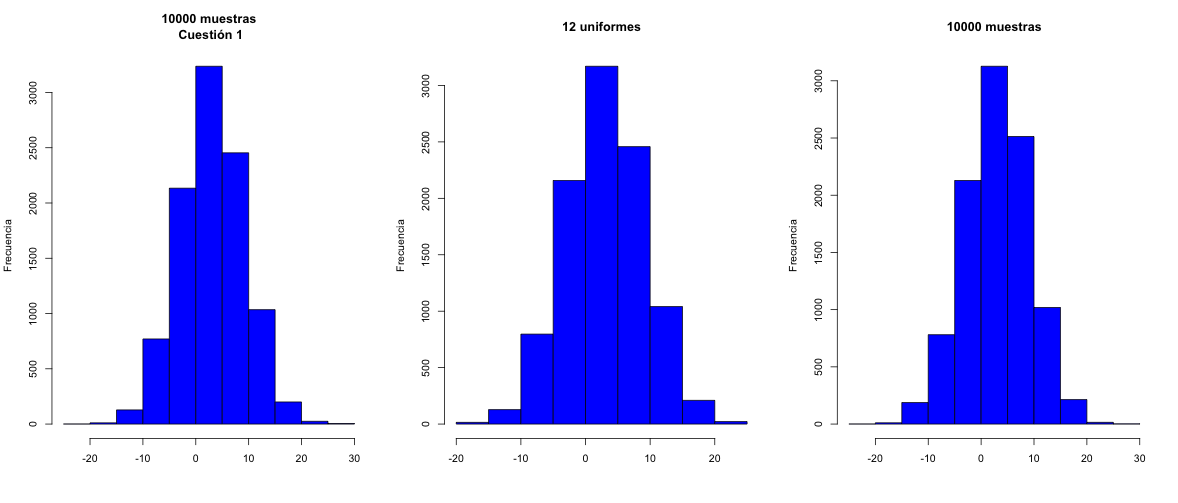
\includegraphics[width=0.8\linewidth]{imagenes/compPlots}
\caption{Comparativa de los histogramas de la distribución normal generados usando distintos métodos}
\label{fig:compPlots}
\end{figure}

Se puede observar que todos los métodos obtienen estadísticos descriptivos muy parecidos a su valor analítico. Esto hace que estemos ante buenos métodos de generación de distribuciones aleatorias, en este caso, una distribución normal.  

\subsection{Cuestión 3}

Usaremos el método de inversión para obtener 10000 muestras de una distribución $\mathcal{E}xp(\lambda = 9)$. El histograma de las muestras generadas se muestra en la Figura~\ref{fig:distExp}.\\

\begin{figure}[htbp!]
\centering
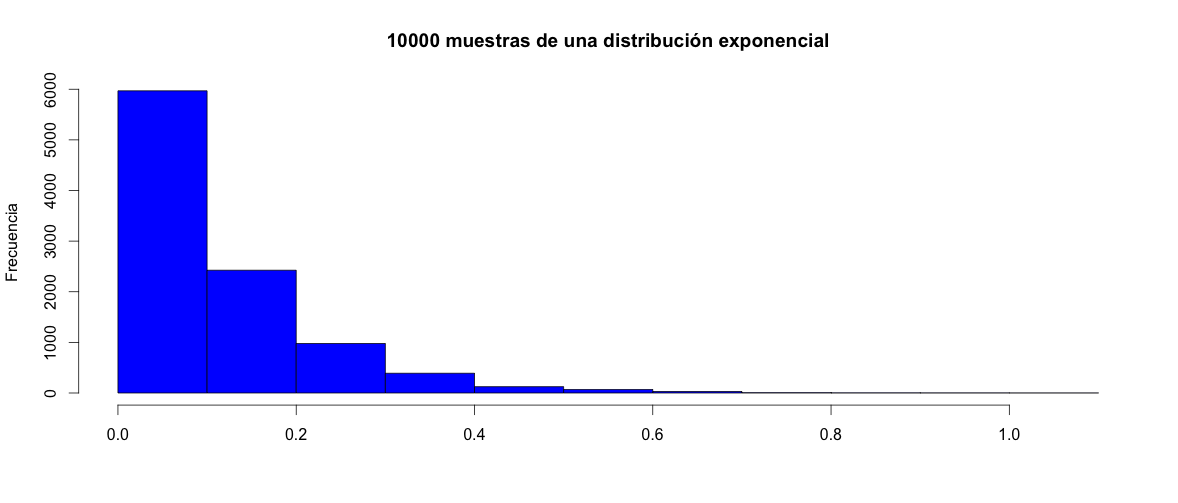
\includegraphics[width=0.8\linewidth]{imagenes/distExp}
\caption{10000 muestras de una distribución exponencial}
\label{fig:distExp}
\end{figure}

Calculamos la media y el coeficiente de variación de la muestra. Recordemos que el coeficiente de variación de la muestra $x$ con media $\mu$ y desviación típica $\sigma$ viene dado por:

\[ \text{CV} = \dfrac{\sigma}{|\mu|} \]


La media de la muestra es de $0.109$ y el coeficiente de variación es de $0.998$.\\

Recordemos que la media de una distribución exponencial de parámetro $\lambda$ es $\frac{1}{\lambda}$. En nuestro caso, $\lambda = 9$ y, $\frac{1}{9} = 0.111 \approx 0.109$.\\

Por otra parte, se tiene que la varianza de una distribución exponencial de parámetro $\lambda$ es $\dfrac{1}{\lambda^2}$, y por tanto, la desviación típica es $\frac{1}{\lambda}$. Por tanto, el coeficiente de variación de una distribución exponencial es 1.\\

Todo lo anterior hace que estemos ante una muy buena aproximación de la distribución exponencial. 

\subsection{Cuestión 4}

A continuación generaremos 10000 muestras de una distribución normal bivariante dado por el vector de medias $\mathbf{\mu} = (\mu_x = 3, \mu_y = 2)$, y matriz de varianzas y covarianzas $\Sigma$, donde $\Sigma$ viene dada por

\[ \Sigma = \left( \begin{array}{cc}
\sigma^2_x = 7^2 & \sigma_{xy}^2 = 4^2\\
\sigma_{xy}^2 = 4^2 & \sigma_y^2 = 5^2
\end{array} \right) \]

En primer lugar, calculamos la matriz de Cholesky de $\Sigma$, obteniéndose,

\[ L = \left( \begin{array}{cc}
2.645751 & 0.000000 \\
1.511858 & 1.647509
\end{array} \right) \]

Se puede comprobar que, efectivamente, $\Sigma = L \cdot L^T$.\\

La muestra generada tiene las siguientes medias:

\[\mu_x = 2.970041, \quad \mu_y = 1.982205\]

Las varianzas son:

\[\sigma_x = 6.911890, \quad \sigma_y = 5.011215 \]

Y la covarianza es:

\[ \sigma_{xy} = 3.97125 \]

De acuerdo a estos resultados, estamos ante a una muy buena aproximación de una distribución normal bivariante.\\

En la Figura~\ref{fig:bivariante} se muestra un scatterplot de las 10000 muestras generadas.\\

\begin{figure}[tbph!]
\centering
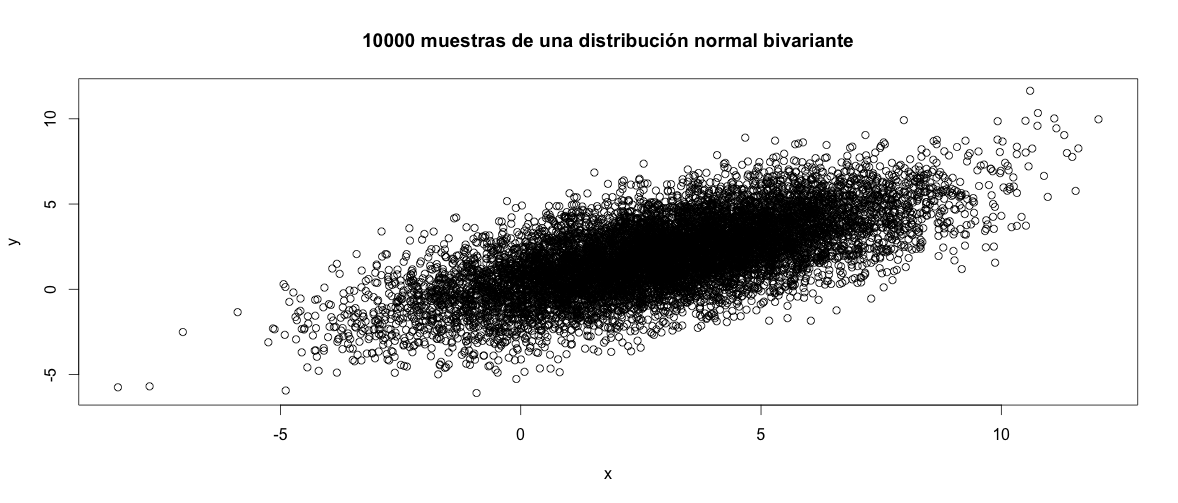
\includegraphics[width=0.8\linewidth]{imagenes/bivariante.png}
\caption{10000 muestras de una distribución normal bivariante}
\label{fig:bivariante}
\end{figure}

Recordemos que la función de densidad de una distribución normal multivariante viene dada por

\[ f(\mathbf{x} = (x_1,\dots, x_n) | \mathbf{\mu}, \Sigma) = \dfrac{1}{2\pi |\Sigma|^{1/2}} \exp \left( -\dfrac{1}{2} (\mathbf{x} - \mathbf{\mu})^T \Sigma^{-1} (\mathbf{x} - \mathbf{\mu}) \right) \] 

La Figura~\ref{fig:bivarianteDen} muestra la función de densidad de la distribución generada.

\begin{figure}[tbph!]
\centering
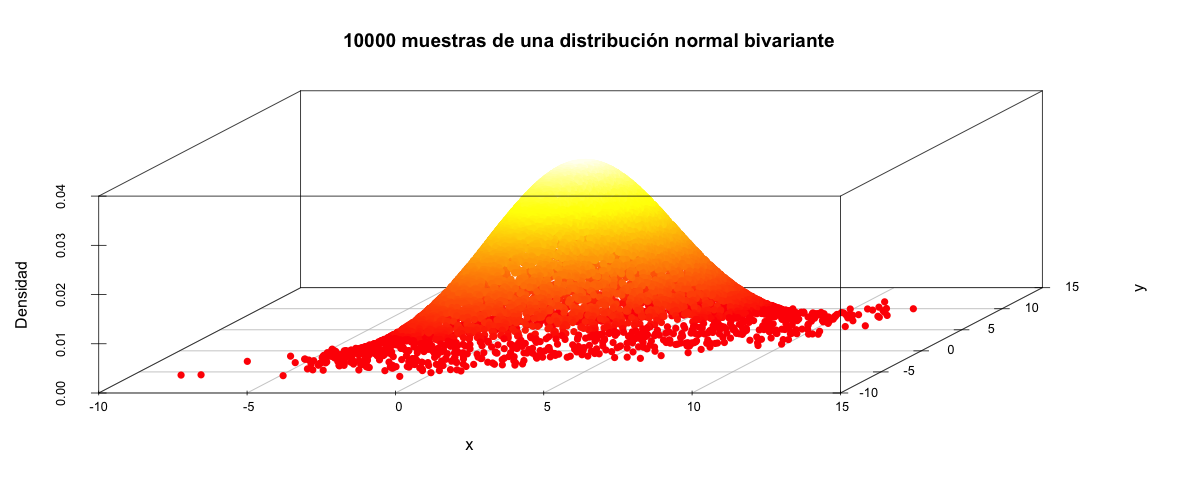
\includegraphics[width=0.8\linewidth]{imagenes/bivarianteDen.png}
\caption{Función de densidad de 10000 muestras de una distribución normal bivariante}
\label{fig:bivarianteDen}
\end{figure}


\section{Conclusiones}
En este caso práctico hemos aprendido a generar distintos tipos de variables aleatorias tanto unidimensionales como multidimensionales, aplicando además, varios métodos de generación: método de las 12 uniformes para la generación de una variable aleatoria normal, el método de inversión para generar variables aleatorias cuya función de distribución es creciente (como en el caso de la distribución exponencial), entre otros.\\

Además, gracias a la gran cantidad de funciones disponibles y la gran capacidad de cálculo de R ha permitido ahorrar mucho tiempo al implementar los distintos métodos de generación de las distintas variables aleatorias.

\newpage

\section{Código R utilizado}

A continuación se muestra el código utilizado para la realización de este caso práctico.

\inputminted{r}{../codigo/caso_ii.R}


\end{document}